Each role identified in the C2 System and described in Section~\ref{sec:roles}, is modeled as a Program Graph(PG) and has their main steps of execution mapped with their variables and constraints.

The actions executing data exchange, i.e., with the '!' and '?' marquees, will be explained in the Section~\ref{sec:cs}. The guard conditions and effects caused by the actions or functions over the variables are described bellow each PG.

\begin{figure}[h!]
\centering
\label{PG001}
\scalebox{.8}{


\tikzset{every picture/.style={line width=0.75pt}} %set default line width to 0.75pt        

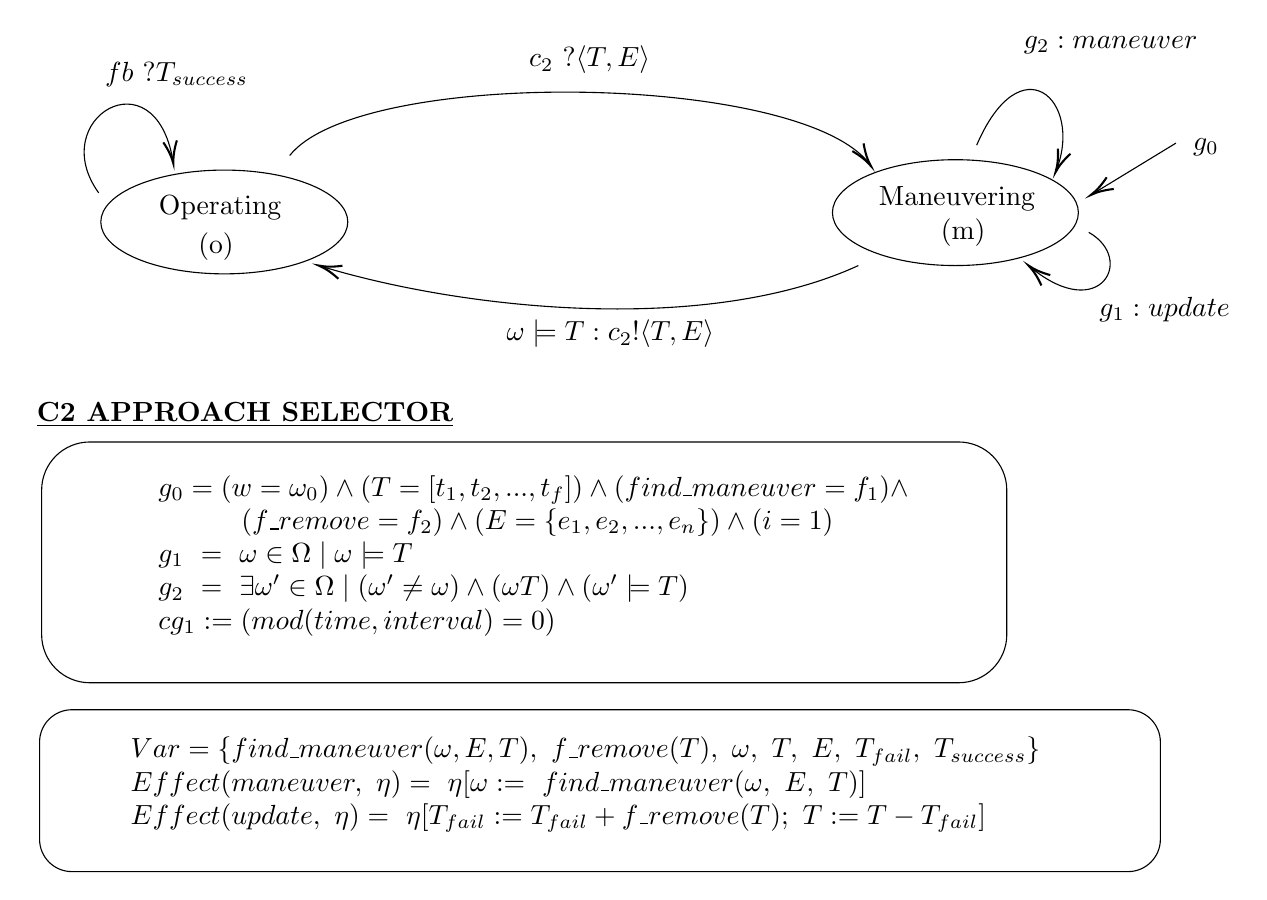
\begin{tikzpicture}[x=0.75pt,y=0.75pt,yscale=-1,xscale=1]
%uncomment if require: \path (0,420); %set diagram left start at 0, and has height of 420

%Curve Lines [id:da9480858267519683] 
\draw    (135.5,66) .. controls (169.16,23.43) and (380.22,25.94) .. (414.52,69.66) ;
\draw [shift={(415.5,71)}, rotate = 235.44] [color={rgb, 255:red, 0; green, 0; blue, 0 }  ][line width=0.75]    (10.93,-3.29) .. controls (6.95,-1.4) and (3.31,-0.3) .. (0,0) .. controls (3.31,0.3) and (6.95,1.4) .. (10.93,3.29)   ;
%Shape: Ellipse [id:dp6594609066072359] 
\draw   (44.5,98) .. controls (44.5,84.19) and (71.14,73) .. (104,73) .. controls (136.86,73) and (163.5,84.19) .. (163.5,98) .. controls (163.5,111.81) and (136.86,123) .. (104,123) .. controls (71.14,123) and (44.5,111.81) .. (44.5,98) -- cycle ;
%Shape: Ellipse [id:dp873836537729809] 
\draw   (397,93.5) .. controls (397,79.42) and (423.53,68) .. (456.25,68) .. controls (488.97,68) and (515.5,79.42) .. (515.5,93.5) .. controls (515.5,107.58) and (488.97,119) .. (456.25,119) .. controls (423.53,119) and (397,107.58) .. (397,93.5) -- cycle ;
%Curve Lines [id:da21020703050779688] 
\draw    (466.5,61) .. controls (487.68,11.75) and (517.59,39.15) .. (505.1,72.47) ;
\draw [shift={(504.5,74)}, rotate = 292.38] [color={rgb, 255:red, 0; green, 0; blue, 0 }  ][line width=0.75]    (10.93,-3.29) .. controls (6.95,-1.4) and (3.31,-0.3) .. (0,0) .. controls (3.31,0.3) and (6.95,1.4) .. (10.93,3.29)   ;
%Curve Lines [id:da14662580418826565] 
\draw    (520.5,103) .. controls (543.16,115.81) and (526.03,147.04) .. (493.02,120.26) ;
\draw [shift={(491.5,119)}, rotate = 400.46000000000004] [color={rgb, 255:red, 0; green, 0; blue, 0 }  ][line width=0.75]    (10.93,-3.29) .. controls (6.95,-1.4) and (3.31,-0.3) .. (0,0) .. controls (3.31,0.3) and (6.95,1.4) .. (10.93,3.29)   ;
%Straight Lines [id:da37650774099478246] 
\draw    (562.5,60) -- (523.21,83.96) ;
\draw [shift={(521.5,85)}, rotate = 328.63] [color={rgb, 255:red, 0; green, 0; blue, 0 }  ][line width=0.75]    (10.93,-3.29) .. controls (6.95,-1.4) and (3.31,-0.3) .. (0,0) .. controls (3.31,0.3) and (6.95,1.4) .. (10.93,3.29)   ;
%Rounded Rect [id:dp20897962983691354] 
\draw   (16,227.2) .. controls (16,214.39) and (26.39,204) .. (39.2,204) -- (457.8,204) .. controls (470.61,204) and (481,214.39) .. (481,227.2) -- (481,296.8) .. controls (481,309.61) and (470.61,320) .. (457.8,320) -- (39.2,320) .. controls (26.39,320) and (16,309.61) .. (16,296.8) -- cycle ;
%Rounded Rect [id:dp6489541210438411] 
\draw   (15,348.6) .. controls (15,339.98) and (21.98,333) .. (30.6,333) -- (539.4,333) .. controls (548.02,333) and (555,339.98) .. (555,348.6) -- (555,395.4) .. controls (555,404.02) and (548.02,411) .. (539.4,411) -- (30.6,411) .. controls (21.98,411) and (15,404.02) .. (15,395.4) -- cycle ;
%Curve Lines [id:da07722007259294938] 
\draw    (43.5,84) .. controls (17.76,48.36) and (70.43,16.64) .. (79.25,68.41) ;
\draw [shift={(79.5,70)}, rotate = 261.57] [color={rgb, 255:red, 0; green, 0; blue, 0 }  ][line width=0.75]    (10.93,-3.29) .. controls (6.95,-1.4) and (3.31,-0.3) .. (0,0) .. controls (3.31,0.3) and (6.95,1.4) .. (10.93,3.29)   ;
%Curve Lines [id:da13961356622291943] 
\draw    (409.5,119) .. controls (335.87,152.83) and (218.68,140.13) .. (150.52,119.31) ;
\draw [shift={(149.5,119)}, rotate = 377.15999999999997] [color={rgb, 255:red, 0; green, 0; blue, 0 }  ][line width=0.75]    (10.93,-3.29) .. controls (6.95,-1.4) and (3.31,-0.3) .. (0,0) .. controls (3.31,0.3) and (6.95,1.4) .. (10.93,3.29)   ;

% Text Node
\draw (102,91) node   [align=left] {Operating};
% Text Node
\draw (457,87) node   [align=left] {Maneuvering};
% Text Node
\draw (280,20) node    {$c_{2} \ ?\langle T,E\rangle $};
% Text Node
\draw (577,62) node    {$g_{0}$};
% Text Node
\draw (557,140) node    {$g_{1} :update$};
% Text Node
\draw (531,13) node    {$g_{2} :maneuver$};
% Text Node
\draw (253,259) node    {$ \begin{array}{l}
g_{0} =( w=\omega _{0}) \land ( T=[ t_{1} ,t_{2} ,...,t_{f}]) \land ( find\_maneuver=f_{1}) \land \\
\ \ \ \ \ \ \ \ \ ( f\_remove=f_{2}) \land ( E=\{e_{1} ,e_{2} ,...,e_{n}\}) \land ( i=1)\\
g_{1} \ =\ \nexists \omega \in \Omega \mid \omega \models T\\
g_{2} \ =\ \exists \omega '\in \Omega \mid ( \omega '\neq \omega ) \land ( \omega \nvDash T) \land ( \omega '\models T)\\
cg_{1} :=( mod( time,interval) =0)
\end{array}$};
% Text Node
\draw (460,103) node   [align=left] {(m)};
% Text Node
\draw (100,110) node   [align=left] {(o)};
% Text Node
\draw (278,369) node    {$ \begin{array}{l}
Var=\{find\_maneuver( \omega ,E,T) ,\ f\_remove( T) ,\ \omega ,\ T,\ E,\ T_{fail} ,\ T_{success}\}\\
Effect( maneuver,\ \eta ) =\ \eta [ \omega :=\ find\_maneuver( \omega ,\ E,\ T)]\\
Effect( update,\ \eta ) =\ \eta [ T_{fail} :=T_{fail} +f\_remove( T) ;\ T:=T-T_{fail}]
\end{array}$};
% Text Node
\draw (81,27) node    {$fb\ ?T_{success}$};
% Text Node
\draw (114,191) node   [align=left] {\textbf{\underline{C2 APPROACH SELECTOR}}};
% Text Node
\draw (290,152) node    {$\omega \models T:c_{2} !\langle T,E\rangle $};


\end{tikzpicture}}
\caption{C2 Approach Selector PG}
\end{figure}

The guard conditions $g_1$ and $g_2$ in the C2 Approach Selector PG have an implicit existential analysis of a C2 approach. It is a previous simple processing to figure out a C2 Approach $\omega$ before evoking the function $find\_maneuver$. This strategy avoids an expensive computation performing the complete C2 Approach finding process twice.


\begin{figure}[h!]
\centering
\label{PG002}
\scalebox{.8}{


\tikzset{every picture/.style={line width=0.75pt}} %set default line width to 0.75pt        

\begin{tikzpicture}[x=0.75pt,y=0.75pt,yscale=-1,xscale=1]
%uncomment if require: \path (0,726); %set diagram left start at 0, and has height of 726

%Curve Lines [id:da9480858267519683] 
\draw    (230.5,181) .. controls (264.16,138.43) and (373.78,135.06) .. (406.05,178.66) ;
\draw [shift={(407,180)}, rotate = 235.44] [color={rgb, 255:red, 0; green, 0; blue, 0 }  ][line width=0.75]    (10.93,-3.29) .. controls (6.95,-1.4) and (3.31,-0.3) .. (0,0) .. controls (3.31,0.3) and (6.95,1.4) .. (10.93,3.29)   ;
%Shape: Ellipse [id:dp6594609066072359] 
\draw   (120.5,208) .. controls (120.5,194.19) and (147.14,183) .. (180,183) .. controls (212.86,183) and (239.5,194.19) .. (239.5,208) .. controls (239.5,221.81) and (212.86,233) .. (180,233) .. controls (147.14,233) and (120.5,221.81) .. (120.5,208) -- cycle ;
%Shape: Ellipse [id:dp873836537729809] 
\draw   (397,201.5) .. controls (397,187.42) and (423.53,176) .. (456.25,176) .. controls (488.97,176) and (515.5,187.42) .. (515.5,201.5) .. controls (515.5,215.58) and (488.97,227) .. (456.25,227) .. controls (423.53,227) and (397,215.58) .. (397,201.5) -- cycle ;
%Curve Lines [id:da14662580418826565] 
\draw    (514.5,424) .. controls (567.96,419.05) and (594.96,385.68) .. (603.25,341.35) ;
\draw [shift={(603.5,340)}, rotate = 460.08] [color={rgb, 255:red, 0; green, 0; blue, 0 }  ][line width=0.75]    (10.93,-3.29) .. controls (6.95,-1.4) and (3.31,-0.3) .. (0,0) .. controls (3.31,0.3) and (6.95,1.4) .. (10.93,3.29)   ;
%Straight Lines [id:da37650774099478246] 
\draw    (232.5,14) -- (263.11,24.36) ;
\draw [shift={(265,25)}, rotate = 198.7] [color={rgb, 255:red, 0; green, 0; blue, 0 }  ][line width=0.75]    (10.93,-3.29) .. controls (6.95,-1.4) and (3.31,-0.3) .. (0,0) .. controls (3.31,0.3) and (6.95,1.4) .. (10.93,3.29)   ;
%Shape: Ellipse [id:dp8139093405894636] 
\draw   (121,419) .. controls (121,405.19) and (147.53,394) .. (180.25,394) .. controls (212.97,394) and (239.5,405.19) .. (239.5,419) .. controls (239.5,432.81) and (212.97,444) .. (180.25,444) .. controls (147.53,444) and (121,432.81) .. (121,419) -- cycle ;
%Shape: Ellipse [id:dp08678607998247811] 
\draw   (391,418) .. controls (391,404.19) and (417.53,393) .. (450.25,393) .. controls (482.97,393) and (509.5,404.19) .. (509.5,418) .. controls (509.5,431.81) and (482.97,443) .. (450.25,443) .. controls (417.53,443) and (391,431.81) .. (391,418) -- cycle ;
%Shape: Ellipse [id:dp07482494496489733] 
\draw   (270,28) .. controls (270,14.75) and (296.53,4) .. (329.25,4) .. controls (361.97,4) and (388.5,14.75) .. (388.5,28) .. controls (388.5,41.25) and (361.97,52) .. (329.25,52) .. controls (296.53,52) and (270,41.25) .. (270,28) -- cycle ;
%Curve Lines [id:da6759956440889884] 
\draw    (123.5,226) .. controls (100.84,271.31) and (108.27,364.16) .. (126.65,401.34) ;
\draw [shift={(127.5,403)}, rotate = 242.18] [color={rgb, 255:red, 0; green, 0; blue, 0 }  ][line width=0.75]    (10.93,-3.29) .. controls (6.95,-1.4) and (3.31,-0.3) .. (0,0) .. controls (3.31,0.3) and (6.95,1.4) .. (10.93,3.29)   ;
%Curve Lines [id:da9572857730465772] 
\draw    (234.22,228.76) .. controls (260.49,268.16) and (260.11,371.42) .. (234.5,399) ;
\draw [shift={(233,227)}, rotate = 54.11] [color={rgb, 255:red, 0; green, 0; blue, 0 }  ][line width=0.75]    (10.93,-3.29) .. controls (6.95,-1.4) and (3.31,-0.3) .. (0,0) .. controls (3.31,0.3) and (6.95,1.4) .. (10.93,3.29)   ;
%Curve Lines [id:da9385545433271328] 
\draw    (517.5,315) .. controls (479.88,326.88) and (463.82,339.74) .. (457.68,385.6) ;
\draw [shift={(457.5,387)}, rotate = 277.28] [color={rgb, 255:red, 0; green, 0; blue, 0 }  ][line width=0.75]    (10.93,-3.29) .. controls (6.95,-1.4) and (3.31,-0.3) .. (0,0) .. controls (3.31,0.3) and (6.95,1.4) .. (10.93,3.29)   ;
%Curve Lines [id:da13526468384837043] 
\draw    (440.5,173) .. controls (426.78,119.1) and (401.54,70) .. (377.94,50.18) ;
\draw [shift={(376.5,49)}, rotate = 398.37] [color={rgb, 255:red, 0; green, 0; blue, 0 }  ][line width=0.75]    (10.93,-3.29) .. controls (6.95,-1.4) and (3.31,-0.3) .. (0,0) .. controls (3.31,0.3) and (6.95,1.4) .. (10.93,3.29)   ;
%Curve Lines [id:da7876400787103589] 
\draw    (267.5,45) .. controls (238.79,63.81) and (213.02,106.14) .. (201.83,170.06) ;
\draw [shift={(201.5,172)}, rotate = 279.61] [color={rgb, 255:red, 0; green, 0; blue, 0 }  ][line width=0.75]    (10.93,-3.29) .. controls (6.95,-1.4) and (3.31,-0.3) .. (0,0) .. controls (3.31,0.3) and (6.95,1.4) .. (10.93,3.29)   ;
%Shape: Ellipse [id:dp538933115831977] 
\draw   (524,310) .. controls (524,296.19) and (550.3,285) .. (582.75,285) .. controls (615.2,285) and (641.5,296.19) .. (641.5,310) .. controls (641.5,323.81) and (615.2,335) .. (582.75,335) .. controls (550.3,335) and (524,323.81) .. (524,310) -- cycle ;
%Curve Lines [id:da663291454681702] 
\draw    (518.5,205) .. controls (566.52,205) and (582.85,245.34) .. (584.42,278.01) ;
\draw [shift={(584.5,280)}, rotate = 268.26] [color={rgb, 255:red, 0; green, 0; blue, 0 }  ][line width=0.75]    (10.93,-3.29) .. controls (6.95,-1.4) and (3.31,-0.3) .. (0,0) .. controls (3.31,0.3) and (6.95,1.4) .. (10.93,3.29)   ;
%Curve Lines [id:da17641910717404863] 
\draw    (413.5,391) .. controls (394.69,323.68) and (299.43,241.66) .. (246.1,216.74) ;
\draw [shift={(244.5,216)}, rotate = 384.36] [color={rgb, 255:red, 0; green, 0; blue, 0 }  ][line width=0.75]    (10.93,-3.29) .. controls (6.95,-1.4) and (3.31,-0.3) .. (0,0) .. controls (3.31,0.3) and (6.95,1.4) .. (10.93,3.29)   ;
%Rounded Rect [id:dp2887172897272543] 
\draw   (6,511.6) .. controls (6,484.76) and (27.76,463) .. (54.6,463) -- (425.4,463) .. controls (452.24,463) and (474,484.76) .. (474,511.6) -- (474,657.4) .. controls (474,684.24) and (452.24,706) .. (425.4,706) -- (54.6,706) .. controls (27.76,706) and (6,684.24) .. (6,657.4) -- cycle ;
%Rounded Rect [id:dp07131134126212679] 
\draw   (479,475.4) .. controls (479,469.1) and (484.1,464) .. (490.4,464) -- (713.6,464) .. controls (719.9,464) and (725,469.1) .. (725,475.4) -- (725,509.6) .. controls (725,515.9) and (719.9,521) .. (713.6,521) -- (490.4,521) .. controls (484.1,521) and (479,515.9) .. (479,509.6) -- cycle ;
%Curve Lines [id:da580151899278355] 
\draw    (113.5,201) .. controls (51.13,189.12) and (89.71,141.96) .. (126.39,184.68) ;
\draw [shift={(127.5,186)}, rotate = 230.57] [color={rgb, 255:red, 0; green, 0; blue, 0 }  ][line width=0.75]    (10.93,-3.29) .. controls (6.95,-1.4) and (3.31,-0.3) .. (0,0) .. controls (3.31,0.3) and (6.95,1.4) .. (10.93,3.29)   ;
%Curve Lines [id:da7513759524359456] 
\draw    (159.5,175) .. controls (143.66,139.36) and (196.43,134.1) .. (179.05,175.72) ;
\draw [shift={(178.5,177)}, rotate = 293.84000000000003] [color={rgb, 255:red, 0; green, 0; blue, 0 }  ][line width=0.75]    (10.93,-3.29) .. controls (6.95,-1.4) and (3.31,-0.3) .. (0,0) .. controls (3.31,0.3) and (6.95,1.4) .. (10.93,3.29)   ;

% Text Node
\draw (181,201) node   [align=left] {Ready};
% Text Node
\draw (457,194) node   [align=left] {Allocating};
% Text Node
\draw (323,167) node    {$T'\ \neq [] :allocate$};
% Text Node
\draw (182,413) node   [align=left] {Updating};
% Text Node
\draw (584,302) node   [align=left] {Notifying};
% Text Node
\draw (330,23) node   [align=left] {Waiting};
% Text Node
\draw (66,304) node    {$c_{1} ?\langle t,e'_{j} \rangle $};
% Text Node
\draw (221,303) node    {$update$};
% Text Node
\draw (487,84) node    {$alloc=[] :c_{2} !\langle T',E'\rangle $};
% Text Node
\draw (188,79) node    {$c_{2} ?\langle T',E'\rangle $};
% Text Node
\draw (452,412) node   [align=left] {Binding};
% Text Node
\draw (599,426) node    {$alloc\neq [] :bind$};
% Text Node
\draw (445,327) node    {$m_{k\ } !\ T'_{k}$};
% Text Node
\draw (596,195) node    {$alloc\neq [] :bind$};
% Text Node
\draw (391,266) node    {$alloc=[] :done$};
% Text Node
\draw (239,592) node    {$ \begin{array}{l}
Var=\{alloc,\ f\_alloc,\ teamStatus,\ T',\ E',\ t,\ e'_{j} ,\ time,\ interval\}\\
alloc=[ \langle \ i,T'_{i} \ \rangle ] ,\ where\ \{i\ \in \mathbb{N} \ |\ 1\ \leq i\ \leq |E|\ \} \ \ and\ T'\ \supseteq \bigcup\limits ^{|E|}_{i=1} T'_{i}\\
Effect( allocate,\ \eta ) =\ \eta [ alloc:=\ f\_alloc( T',\ E')]\\
Effect( bind,\ \eta ) =\ \eta [ \ \langle k,T'_{k} \rangle :=head( alloc) ;\ alloc:=tail( alloc) \ ]\\
Effect( update,\ \eta ) =\eta [ \ T':=T'\cup \ [ t] \ ;\ E'=E'( e_{j} /e'_{\ }_{j})]\\
Effect( done,\eta ) =\eta [ \ T':=[] \ ]\\
Effect( addTask,\eta ) =\eta [ \ T':=T'+[ t'_{1} ,t'_{2} ,\ ...,\ t'_{k}] \ ]\\
Effect( ping,\eta ) =\eta [ \ E':=teamStatus( E') \ ]\\
\end{array}$};
% Text Node
\draw (219,8) node    {$g_{0}$};
% Text Node
\draw (331,39) node   [align=left] {(w)};
% Text Node
\draw (180,217) node   [align=left] {(r)};
% Text Node
\draw (458,211) node   [align=left] {(a)};
% Text Node
\draw (183,430) node   [align=left] {(u)};
% Text Node
\draw (450,428) node   [align=left] {(b)};
% Text Node
\draw (582,320) node   [align=left] {(n)};
% Text Node
\draw (604,500) node    {$ \begin{array}{l}
g_{0} :=( T'=[]) \ \land ( f\_alloc\ =\ f_{x})\\
cg_{1} :=( mod( time,interval) =0)\\
\end{array}$};
% Text Node
\draw (75,155) node    {$cg_{1} :ping$};
% Text Node
\draw (163,134) node    {$addTask$};


\end{tikzpicture}}
\caption{Task Allocator PG}
\end{figure}


\begin{figure}[h!]
\centering
\label{PG003}
\scalebox{.8}{

\tikzset{every picture/.style={line width=0.75pt}} %set default line width to 0.75pt        

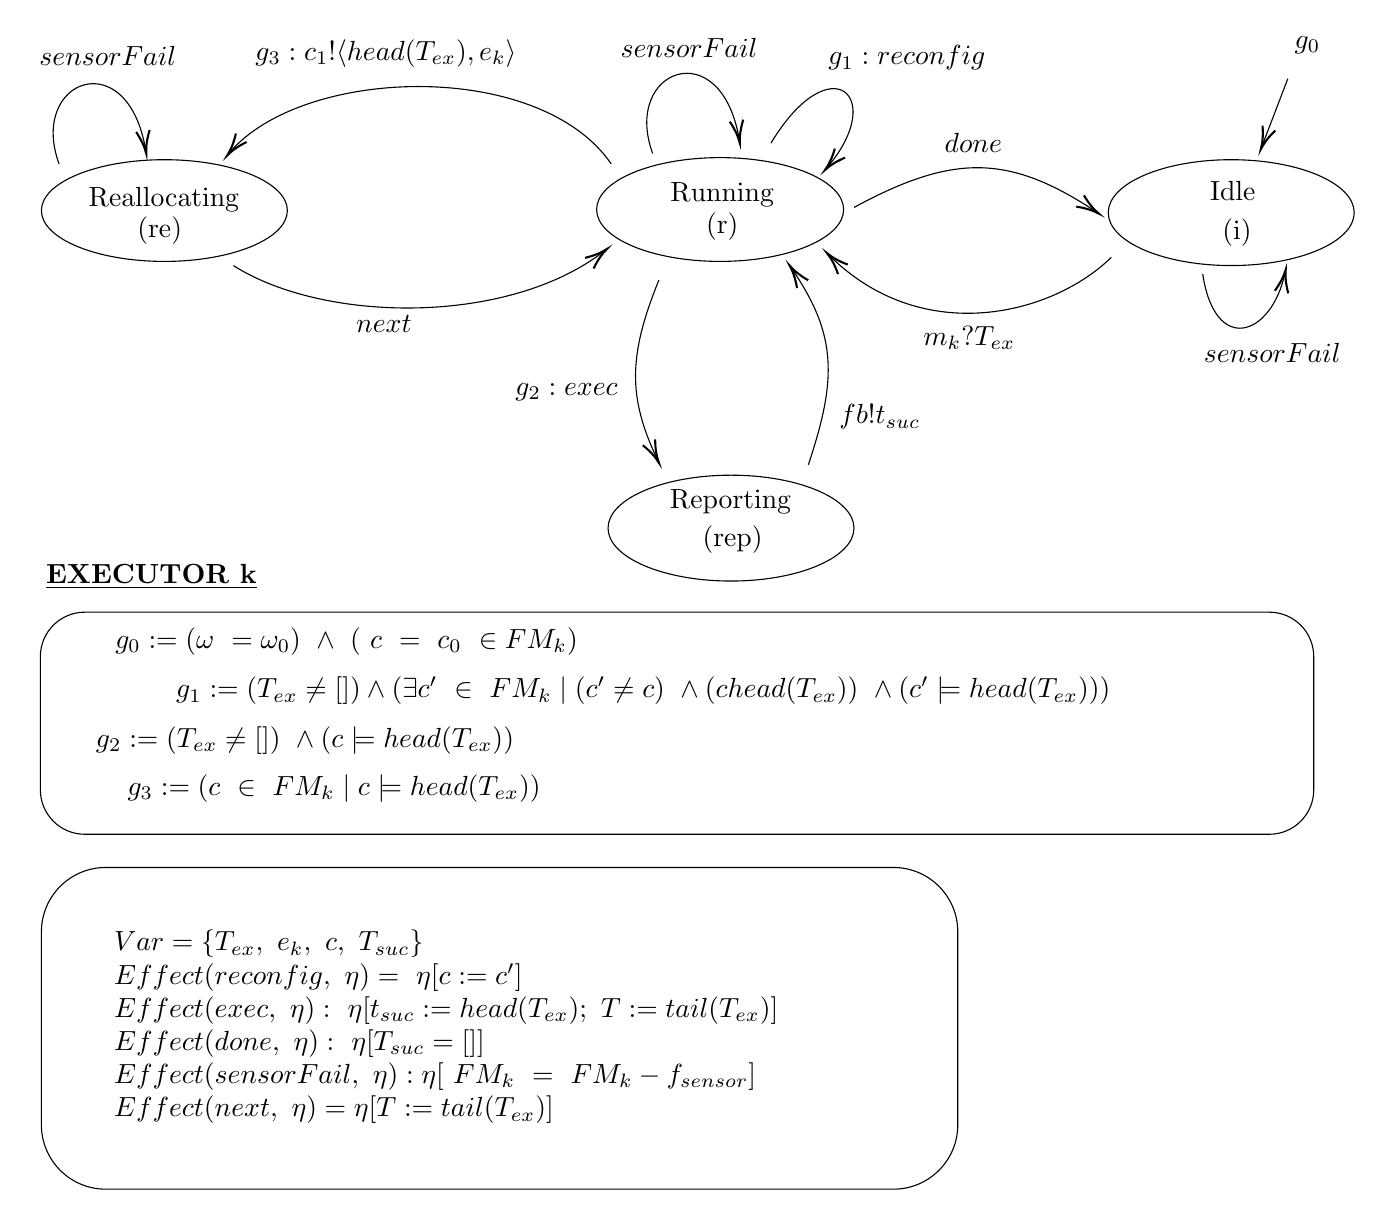
\begin{tikzpicture}[x=0.75pt,y=0.75pt,yscale=-1,xscale=1]
%uncomment if require: \path (0,582); %set diagram left start at 0, and has height of 582

%Curve Lines [id:da9480858267519683] 
\draw    (385.5,222) .. controls (399.29,180.63) and (399.5,159.63) .. (377.52,127.48) ;
\draw [shift={(376.5,126)}, rotate = 415.12] [color={rgb, 255:red, 0; green, 0; blue, 0 }  ][line width=0.75]    (10.93,-3.29) .. controls (6.95,-1.4) and (3.31,-0.3) .. (0,0) .. controls (3.31,0.3) and (6.95,1.4) .. (10.93,3.29)   ;
%Shape: Ellipse [id:dp6594609066072359] 
\draw   (283.5,99) .. controls (283.5,85.19) and (310.14,74) .. (343,74) .. controls (375.86,74) and (402.5,85.19) .. (402.5,99) .. controls (402.5,112.81) and (375.86,124) .. (343,124) .. controls (310.14,124) and (283.5,112.81) .. (283.5,99) -- cycle ;
%Shape: Ellipse [id:dp873836537729809] 
\draw   (530,100.5) .. controls (530,86.42) and (556.53,75) .. (589.25,75) .. controls (621.97,75) and (648.5,86.42) .. (648.5,100.5) .. controls (648.5,114.58) and (621.97,126) .. (589.25,126) .. controls (556.53,126) and (530,114.58) .. (530,100.5) -- cycle ;
%Curve Lines [id:da21020703050779688] 
\draw    (367.5,67) .. controls (396.21,19.48) and (423.94,44.49) .. (394.41,78.95) ;
\draw [shift={(393.5,80)}, rotate = 311.53] [color={rgb, 255:red, 0; green, 0; blue, 0 }  ][line width=0.75]    (10.93,-3.29) .. controls (6.95,-1.4) and (3.31,-0.3) .. (0,0) .. controls (3.31,0.3) and (6.95,1.4) .. (10.93,3.29)   ;
%Straight Lines [id:da37650774099478246] 
\draw    (616.5,36) -- (604.21,68.13) ;
\draw [shift={(603.5,70)}, rotate = 290.92] [color={rgb, 255:red, 0; green, 0; blue, 0 }  ][line width=0.75]    (10.93,-3.29) .. controls (6.95,-1.4) and (3.31,-0.3) .. (0,0) .. controls (3.31,0.3) and (6.95,1.4) .. (10.93,3.29)   ;
%Shape: Ellipse [id:dp02234558999259495] 
\draw   (16,99.5) .. controls (16,85.97) and (42.53,75) .. (75.25,75) .. controls (107.97,75) and (134.5,85.97) .. (134.5,99.5) .. controls (134.5,113.03) and (107.97,124) .. (75.25,124) .. controls (42.53,124) and (16,113.03) .. (16,99.5) -- cycle ;
%Curve Lines [id:da2517277021570281] 
\draw    (290.5,77) .. controls (255.85,26.51) and (141.81,29.93) .. (106.54,71.72) ;
\draw [shift={(105.5,73)}, rotate = 308.33000000000004] [color={rgb, 255:red, 0; green, 0; blue, 0 }  ][line width=0.75]    (10.93,-3.29) .. controls (6.95,-1.4) and (3.31,-0.3) .. (0,0) .. controls (3.31,0.3) and (6.95,1.4) .. (10.93,3.29)   ;
%Curve Lines [id:da851947022127026] 
\draw    (108.5,126) .. controls (152.06,153.72) and (240.7,154.98) .. (287.11,119.1) ;
\draw [shift={(288.5,118)}, rotate = 501.19] [color={rgb, 255:red, 0; green, 0; blue, 0 }  ][line width=0.75]    (10.93,-3.29) .. controls (6.95,-1.4) and (3.31,-0.3) .. (0,0) .. controls (3.31,0.3) and (6.95,1.4) .. (10.93,3.29)   ;
%Curve Lines [id:da05773774536505705] 
\draw    (531.5,122) .. controls (503.29,149.72) and (440.77,165.68) .. (395.86,121.36) ;
\draw [shift={(394.5,120)}, rotate = 405.63] [color={rgb, 255:red, 0; green, 0; blue, 0 }  ][line width=0.75]    (10.93,-3.29) .. controls (6.95,-1.4) and (3.31,-0.3) .. (0,0) .. controls (3.31,0.3) and (6.95,1.4) .. (10.93,3.29)   ;
%Rounded Rect [id:dp5913972444482631] 
\draw   (15.5,314.4) .. controls (15.5,302.58) and (25.08,293) .. (36.9,293) -- (607.6,293) .. controls (619.42,293) and (629,302.58) .. (629,314.4) -- (629,378.6) .. controls (629,390.42) and (619.42,400) .. (607.6,400) -- (36.9,400) .. controls (25.08,400) and (15.5,390.42) .. (15.5,378.6) -- cycle ;
%Rounded Rect [id:dp9206164489184118] 
\draw   (16,447) .. controls (16,429.88) and (29.88,416) .. (47,416) -- (426.5,416) .. controls (443.62,416) and (457.5,429.88) .. (457.5,447) -- (457.5,540) .. controls (457.5,557.12) and (443.62,571) .. (426.5,571) -- (47,571) .. controls (29.88,571) and (16,557.12) .. (16,540) -- cycle ;
%Curve Lines [id:da46585089178877326] 
\draw    (24.5,77) .. controls (9.65,36.41) and (57.53,18.36) .. (66.25,70.4) ;
\draw [shift={(66.5,72)}, rotate = 261.57] [color={rgb, 255:red, 0; green, 0; blue, 0 }  ][line width=0.75]    (10.93,-3.29) .. controls (6.95,-1.4) and (3.31,-0.3) .. (0,0) .. controls (3.31,0.3) and (6.95,1.4) .. (10.93,3.29)   ;
%Curve Lines [id:da24525569786800605] 
\draw    (575.5,130) .. controls (581.38,169.2) and (608.39,160.38) .. (615.11,129.89) ;
\draw [shift={(615.5,128)}, rotate = 460.62] [color={rgb, 255:red, 0; green, 0; blue, 0 }  ][line width=0.75]    (10.93,-3.29) .. controls (6.95,-1.4) and (3.31,-0.3) .. (0,0) .. controls (3.31,0.3) and (6.95,1.4) .. (10.93,3.29)   ;
%Curve Lines [id:da5617910694928671] 
\draw    (310.5,72) .. controls (295.65,31.41) and (343.53,13.36) .. (352.25,65.4) ;
\draw [shift={(352.5,67)}, rotate = 261.57] [color={rgb, 255:red, 0; green, 0; blue, 0 }  ][line width=0.75]    (10.93,-3.29) .. controls (6.95,-1.4) and (3.31,-0.3) .. (0,0) .. controls (3.31,0.3) and (6.95,1.4) .. (10.93,3.29)   ;
%Shape: Ellipse [id:dp893416141673501] 
\draw   (289,252.5) .. controls (289,238.42) and (315.53,227) .. (348.25,227) .. controls (380.97,227) and (407.5,238.42) .. (407.5,252.5) .. controls (407.5,266.58) and (380.97,278) .. (348.25,278) .. controls (315.53,278) and (289,266.58) .. (289,252.5) -- cycle ;
%Curve Lines [id:da2982425830385871] 
\draw    (313.5,133) .. controls (298.72,169.45) and (298.5,189.4) .. (312.84,219.61) ;
\draw [shift={(313.5,221)}, rotate = 244.18] [color={rgb, 255:red, 0; green, 0; blue, 0 }  ][line width=0.75]    (10.93,-3.29) .. controls (6.95,-1.4) and (3.31,-0.3) .. (0,0) .. controls (3.31,0.3) and (6.95,1.4) .. (10.93,3.29)   ;
%Curve Lines [id:da08998093824564413] 
\draw    (407.5,98) .. controls (455.02,72.26) and (481.96,72) .. (524.21,100.14) ;
\draw [shift={(525.5,101)}, rotate = 214] [color={rgb, 255:red, 0; green, 0; blue, 0 }  ][line width=0.75]    (10.93,-3.29) .. controls (6.95,-1.4) and (3.31,-0.3) .. (0,0) .. controls (3.31,0.3) and (6.95,1.4) .. (10.93,3.29)   ;

% Text Node
\draw (344,92) node   [align=left] {Running};
% Text Node
\draw (590,90) node   [align=left] {Idle};
% Text Node
\draw (420,199) node    {$fb!t_{suc}$};
% Text Node
\draw (182,24) node    {$g_{3} :c_{1} !\langle head( T_{ex}) ,e_{k} \rangle $};
% Text Node
\draw (463,161) node    {$m_{k} ?T_{ex}$};
% Text Node
\draw (75,94) node   [align=left] {Reallocating};
% Text Node
\draw (181,154) node    {$next$};
% Text Node
\draw (306,331) node    {$g_{1} :=( T_{ex} \neq []) \land ( \exists c'\ \in \ \llbracket FM_{k} \rrbracket \mid ( c'\neq c) \ \land ( c\nvDash head( T_{ex})) \ \land ( c'\models head( T_{ex})))$};
% Text Node
\draw (433,26) node    {$g_{1} :reconfig$};
% Text Node
\draw (269,187) node    {$g_{2} :exec$};
% Text Node
\draw (143,355) node    {$g_{2} :=( T_{ex} \neq []) \ \land ( c\models head( T_{ex}))$};
% Text Node
\draw (152,461) node    {$ \begin{array}{l}
\end{array}$};
% Text Node
\draw (211,493) node    {$ \begin{array}{l}
Var=\{T_{ex} ,\ e_{k} ,\ c,\ T_{suc}\}\\
Effect( reconfig,\ \eta ) =\ \eta [ c:=c']\\
Effect( exec,\ \eta ) :\ \eta [ t_{suc} :=head( T_{ex}) ;\ T:=tail( T_{ex})]\\
Effect( done,\ \eta ) :\ \eta [ T_{suc} =[]]\\
Effect( sensorFail,\ \eta ) :\eta [ \ FM_{k} \ =\ FM_{k} -f_{sensor}]\\
Effect( next,\ \eta ) =\eta [ T:=tail( T_{ex})]
\end{array}$};
% Text Node
\draw (73,109) node   [align=left] {(re)};
% Text Node
\draw (344,107) node   [align=left] {(r)};
% Text Node
\draw (592,110) node   [align=left] {(i)};
% Text Node
\draw (626,20) node    {$g_{0}$};
% Text Node
\draw (157,378) node    {$g_{3} :=( \nexists c\ \in \ \llbracket FM_{k} \rrbracket \mid c\models head( T_{ex}))$};
% Text Node
\draw (163,307) node    {$g_{0} :=( \omega \ =\omega _{0}) \ \land \ ( \ c\ =\ c_{0} \ \in \llbracket FM_{k} \rrbracket )$};
% Text Node
\draw (48,25) node    {$sensorFail$};
% Text Node
\draw (609,168) node    {$sensorFail$};
% Text Node
\draw (465,67) node    {$done$};
% Text Node
\draw (328,21) node    {$sensorFail$};
% Text Node
\draw (348,240) node   [align=left] {Reporting};
% Text Node
\draw (349,258) node   [align=left] {(rep)};
% Text Node
\draw (69,276) node   [align=left] {\textbf{\underline{EXECUTOR k}}};


\end{tikzpicture}}
\caption{Executor PG}
\end{figure}

It can be necessary to implement a monitoring mechanism able to figure out which members are online and any configuration modification. This procedure can be executed through a ping protocol following a time interval $\Delta t$. The action will be called if the condition showed by Equation \ref{eq001} is satisfied.

\begin{center}
\begin{equation}
\label{eq001}
if\ mod(current_time, \Delta t)=0
\end{equation}
\end{center}